\begin{figure}[htbp]
\centering
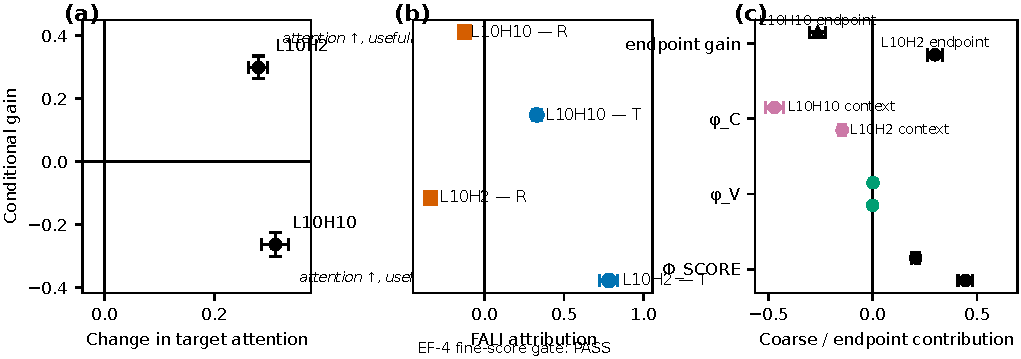
\includegraphics[width=\textwidth]{figures/Fig4.pdf}
\caption{GPT-2 IOI separates attention adaptation from positive functional recruitment. (a) L10H2 and L10H10 both increase attention to the indirect-object target after ablation of the canonical primary Name Movers, but their conditional gains have opposite signs. (b) Both heads show positive target-score and negative rival-score FALI contributions, while $O$ and $V$ remain near zero on the plotted scale. (c) Coarse score/value/context accounting explains the difference: L10H10 retains a positive SCORE contribution, but its negative surrounding-context contribution outweighs it and yields negative conditional gain. Points are balanced means; intervals are hierarchical 95\% bootstrap confidence intervals}
\label{fig:gpt2-attention-recruitment}
\end{figure}
